% Options for packages loaded elsewhere
% Options for packages loaded elsewhere
\PassOptionsToPackage{unicode}{hyperref}
\PassOptionsToPackage{hyphens}{url}
%
\documentclass[
  ignorenonframetext,
  aspectratio=169,
]{beamer}
\newif\ifbibliography
\usepackage{pgfpages}
\setbeamertemplate{caption}[numbered]
\setbeamertemplate{caption label separator}{: }
\setbeamercolor{caption name}{fg=normal text.fg}
\beamertemplatenavigationsymbolsempty
% remove section numbering
\setbeamertemplate{part page}{
  \centering
  \begin{beamercolorbox}[sep=16pt,center]{part title}
    \usebeamerfont{part title}\insertpart\par
  \end{beamercolorbox}
}
\setbeamertemplate{section page}{
  \centering
  \begin{beamercolorbox}[sep=12pt,center]{section title}
    \usebeamerfont{section title}\insertsection\par
  \end{beamercolorbox}
}
\setbeamertemplate{subsection page}{
  \centering
  \begin{beamercolorbox}[sep=8pt,center]{subsection title}
    \usebeamerfont{subsection title}\insertsubsection\par
  \end{beamercolorbox}
}
% Prevent slide breaks in the middle of a paragraph
\widowpenalties 1 10000
\raggedbottom
\usepackage{iftex}
\ifPDFTeX
  \usepackage[T1]{fontenc}
  \usepackage[utf8]{inputenc}
  \usepackage{textcomp} % provide euro and other symbols
\else % if luatex or xetex
  \usepackage{unicode-math} % this also loads fontspec
  \defaultfontfeatures{Scale=MatchLowercase}
  \defaultfontfeatures[\rmfamily]{Ligatures=TeX,Scale=1}
\fi
\usepackage{lmodern}

\usetheme[]{metropolis}
\ifPDFTeX\else
  % xetex/luatex font selection
\fi
% Use upquote if available, for straight quotes in verbatim environments
\IfFileExists{upquote.sty}{\usepackage{upquote}}{}
\IfFileExists{microtype.sty}{% use microtype if available
  \usepackage[]{microtype}
  \UseMicrotypeSet[protrusion]{basicmath} % disable protrusion for tt fonts
}{}
\makeatletter
\@ifundefined{KOMAClassName}{% if non-KOMA class
  \IfFileExists{parskip.sty}{%
    \usepackage{parskip}
  }{% else
    \setlength{\parindent}{0pt}
    \setlength{\parskip}{6pt plus 2pt minus 1pt}}
}{% if KOMA class
  \KOMAoptions{parskip=half}}
\makeatother


\usepackage{longtable,booktabs,array}
\usepackage{calc} % for calculating minipage widths
\usepackage{caption}
% Make caption package work with longtable
\makeatletter
\def\fnum@table{\tablename~\thetable}
\makeatother
\usepackage{graphicx}
\makeatletter
\newsavebox\pandoc@box
\newcommand*\pandocbounded[1]{% scales image to fit in text height/width
  \sbox\pandoc@box{#1}%
  \Gscale@div\@tempa{\textheight}{\dimexpr\ht\pandoc@box+\dp\pandoc@box\relax}%
  \Gscale@div\@tempb{\linewidth}{\wd\pandoc@box}%
  \ifdim\@tempb\p@<\@tempa\p@\let\@tempa\@tempb\fi% select the smaller of both
  \ifdim\@tempa\p@<\p@\scalebox{\@tempa}{\usebox\pandoc@box}%
  \else\usebox{\pandoc@box}%
  \fi%
}
% Set default figure placement to htbp
\def\fps@figure{htbp}
\makeatother





\setlength{\emergencystretch}{3em} % prevent overfull lines

\providecommand{\tightlist}{%
  \setlength{\itemsep}{0pt}\setlength{\parskip}{0pt}}



 


% ============================================================
%  Econ 2203 — Beamer Metropolis Theme Preamble
%  Course: International Trade and Policy in Agriculture
%  Instructor: Nithin M, Department of Development Economics
% ============================================================

% MUST be first: load Metropolis theme before \metroset and colour overrides
\usetheme{metropolis}

% Only load packages not already provided by pandoc's beamer template
\usepackage{amsmath,amssymb}

% ---- Brand colours -----------------------------------------
\definecolor{brandblue}{HTML}{012169}
\definecolor{brandgold}{HTML}{B9975B}
\definecolor{lightblue}{HTML}{E8EDF5}

% ---- Metropolis colour overrides ---------------------------
% Main palette
\setbeamercolor{normal text}{fg=black,bg=white}
\setbeamercolor{background canvas}{bg=white}
\setbeamercolor{alerted text}{fg=brandgold}
\setbeamercolor{example text}{fg=brandblue!70!black}

% Title slide
\setbeamercolor{title}{fg=white,bg=brandblue}
\setbeamercolor{subtitle}{fg=brandgold}
\setbeamercolor{author}{fg=white}
\setbeamercolor{institute}{fg=brandgold!80!white}
\setbeamercolor{date}{fg=white}
\setbeamercolor{title page header}{fg=white,bg=brandblue}

% Frametitle bar
\setbeamercolor{frametitle}{fg=white,bg=brandblue}

% Progress bar → gold
\setbeamercolor{progress bar}{fg=brandgold,bg=brandblue!30}
\setbeamercolor{title separator}{fg=brandgold}
\setbeamercolor{progress bar in head/foot}{fg=brandgold,bg=brandblue!20}
\setbeamercolor{progress bar in section page}{fg=brandgold,bg=brandblue!20}

% Blocks
\setbeamercolor{block title}{bg=brandblue,fg=white}
\setbeamercolor{block body}{bg=lightblue,fg=black}
\setbeamercolor{block title alerted}{bg=brandgold,fg=white}
\setbeamercolor{block body alerted}{bg=brandgold!12,fg=black}
\setbeamercolor{block title example}{bg=brandblue!70!black,fg=white}
\setbeamercolor{block body example}{bg=brandblue!8,fg=black}

% Structure / lists
\setbeamercolor{structure}{fg=brandblue}
\setbeamercolor{section in toc}{fg=brandblue}
\setbeamercolor{itemize item}{fg=brandblue}
\setbeamercolor{itemize subitem}{fg=brandgold}
\setbeamercolor{enumerate item}{fg=brandblue}
\setbeamercolor{description item}{fg=brandblue}

% ---- Metropolis options ------------------------------------
\metroset{
  progressbar    = frametitle,   % gold bar under frametitle
  sectionpage    = none,
  numbering      = fraction,
  block          = fill
}

% ---- Fonts (Metropolis uses Fira Sans; fallback gracefully) -
\setbeamerfont{title}{size=\Large,series=\bfseries}
\setbeamerfont{subtitle}{size=\normalsize,series=\mdseries}
\setbeamerfont{frametitle}{size=\large,series=\bfseries}
\setbeamerfont{block title}{size=\normalsize,series=\bfseries}
\setbeamerfont{caption}{size=\footnotesize}

% ---- Footer: lecture title + course + slide number ----------
\setbeamertemplate{footline}{%
  \begin{beamercolorbox}[wd=\paperwidth,ht=2.0ex,dp=1ex]{footline}%
    \hspace{0.8em}%
    {\footnotesize\color{brandblue!60}%
      \insertshorttitle
      \hfill Nithin M \hfill
      \insertframenumber{}/\inserttotalframenumber\hspace{0.8em}}%
  \end{beamercolorbox}%
}

% ---- Misc --------------------------------------------------
\setlength{\parskip}{2pt}
\setbeamertemplate{navigation symbols}{}

% tighter column sep for side-by-side content
\setlength{\columnsep}{0.8em}

% ---- Max 6 lines per slide: compact list typesetting -------
% Smaller fonts at each list depth
\setbeamerfont{itemize/enumerate body}{size=\small}
\setbeamerfont{itemize/enumerate subbody}{size=\footnotesize}
\setbeamerfont{itemize/enumerate subsubbody}{size=\scriptsize}

% Tight vertical spacing injected at the start of each list level
\setbeamertemplate{itemize/enumerate body begin}{%
  \setlength{\itemsep}{3pt}\setlength{\parsep}{0pt}}
\setbeamertemplate{itemize/enumerate subbody begin}{%
  \setlength{\itemsep}{2pt}\setlength{\parsep}{0pt}}
\setbeamertemplate{itemize/enumerate subsubbody begin}{%
  \setlength{\itemsep}{1pt}\setlength{\parsep}{0pt}}

% Global safety net: default frame shrink = 10 %
% \beamer@shrinkfalse is called ONCE in beamer's frame init (line 438 of
% beamerbaseframe.sty) before the user's options are processed (line 444).
% By redefining it we inject shrink=10 right after the reset; if the frame
% explicitly specifies [shrink=X], the later \setkeys call overrides it.
\makeatletter
\let\beamer@orig@shrinkfalse\beamer@shrinkfalse
\def\beamer@shrinkfalse{%
  \beamer@orig@shrinkfalse
  \setkeys{beamerframe}{shrink=10}}
\makeatother

% Fix: make \label truly robust in moving arguments.
% Quarto wraps figure labels inside captions; Metropolis expands them
% in batchmode causing a crash. DeclareRobustCommand prevents expansion.
\makeatletter
\let\quarto@originallabel\label
\DeclareRobustCommand*{\label}[1]{\quarto@originallabel{#1}}
\makeatother

% Prevent figures from overflowing Beamer frames.
% width=\linewidth: scale to text width (already Quarto default);
% height=0.6\textheight: cap height so figures never push past the frame bottom.
% keepaspectratio: never distort — whichever constraint binds first wins.
\setkeys{Gin}{width=\linewidth,height=0.55\textheight,keepaspectratio}
\makeatletter
\@ifpackageloaded{caption}{}{\usepackage{caption}}
\AtBeginDocument{%
\ifdefined\contentsname
  \renewcommand*\contentsname{Table of contents}
\else
  \newcommand\contentsname{Table of contents}
\fi
\ifdefined\listfigurename
  \renewcommand*\listfigurename{List of Figures}
\else
  \newcommand\listfigurename{List of Figures}
\fi
\ifdefined\listtablename
  \renewcommand*\listtablename{List of Tables}
\else
  \newcommand\listtablename{List of Tables}
\fi
\ifdefined\figurename
  \renewcommand*\figurename{Figure}
\else
  \newcommand\figurename{Figure}
\fi
\ifdefined\tablename
  \renewcommand*\tablename{Table}
\else
  \newcommand\tablename{Table}
\fi
}
\@ifpackageloaded{float}{}{\usepackage{float}}
\floatstyle{ruled}
\@ifundefined{c@chapter}{\newfloat{codelisting}{h}{lop}}{\newfloat{codelisting}{h}{lop}[chapter]}
\floatname{codelisting}{Listing}
\newcommand*\listoflistings{\listof{codelisting}{List of Listings}}
\makeatother
\makeatletter
\makeatother
\makeatletter
\@ifpackageloaded{caption}{}{\usepackage{caption}}
\@ifpackageloaded{subcaption}{}{\usepackage{subcaption}}
\makeatother

\usepackage{bookmark}
\IfFileExists{xurl.sty}{\usepackage{xurl}}{} % add URL line breaks if available
\urlstyle{same}
\hypersetup{
  pdftitle={Lecture 8: Protectionism II --- Subsidies, Dumping \& Cartels},
  pdfauthor={Nithin M},
  hidelinks,
  pdfcreator={LaTeX via pandoc}}


\title[L8 \textbar{} Protectionism II]{Lecture 8: Protectionism II ---
Subsidies, Dumping \& Cartels}
\subtitle{Econ 2203 \textbar{} International Trade and Policy in
Agriculture}
\author{Nithin M}
\date{2026-06-13}
\institute{Department of Development Economics}

\begin{document}
\frame{\titlepage}


\begin{frame}{Recap: Tariffs and Quotas}
\phantomsection\label{recap-tariffs-and-quotas}
\textbf{Last lecture (L7):} border instruments that restrict imports

\begin{itemize}
\tightlist
\item
  \textbf{Tariffs} → raise domestic price \(P_d = P_w(1+t)\), generate
  revenue \(t \cdot M\), DWL \(= b + d\)
\item
  \textbf{Quotas} → fix import volume \(\bar{M}\); quota rents go to
  licence holders
\item
  India: high bound tariffs, TRQs, tariff ``water'' provides policy
  flexibility
\end{itemize}

\textbf{Today:} instruments that \emph{push} exports or distort domestic
production: export subsidies, dumping, VERs, and cartels.

\textbf{Political economy insight:} Tariffs/quotas protect
import-competing producers. Export subsidies protect exporting
producers. Both are driven by producer lobbying --- even though
consumers and taxpayers bear the cost:
\(\text{Producer surplus gain} > \text{Consumer + taxpayer loss?}\) ---
usually \textbf{no} in aggregate, but politically organised producers
win.
\end{frame}

\begin{frame}{What Is an Export Subsidy?}
\phantomsection\label{what-is-an-export-subsidy}
An \textbf{export subsidy} is a direct government payment \(s\) per unit
exported.

\textbf{Mechanism:} Domestic producers can sell abroad at \(P_w\) and
receive subsidy \(s\), so net return = \(P_w + s\) → \textbf{domestic
price rises to} \(P_d = P_w + s\).

\begin{longtable}[]{@{}lll@{}}
\toprule\noalign{}
Group & Direction & Why \\
\midrule\noalign{}
\endhead
Producers & \textbf{Gain} & Higher domestic price \\
Consumers & \textbf{Lose} & Pay \(P_d > P_w\) \\
Government & \textbf{Pays} & \(s \times \text{export volume}\) \\
\bottomrule\noalign{}
\end{longtable}

\textbf{Price wedge identity:} \(\boxed{P_d = P_w + s}\);
\(Q_s \uparrow\), \(Q_d \downarrow\), Exports \(= Q_s - Q_d \uparrow\)

\textbf{Large-country effect:} World price \(P_w\) falls as export
supply increases → terms of trade deteriorate → exporter loses even
more:
\(\Delta W_{\text{large country}} < \Delta W_{\text{small country}} < 0\)
\end{frame}

\begin{frame}{Export Subsidy: Welfare Diagram}
\phantomsection\label{export-subsidy-welfare-diagram}
\begin{figure}

\centering{

\pandocbounded{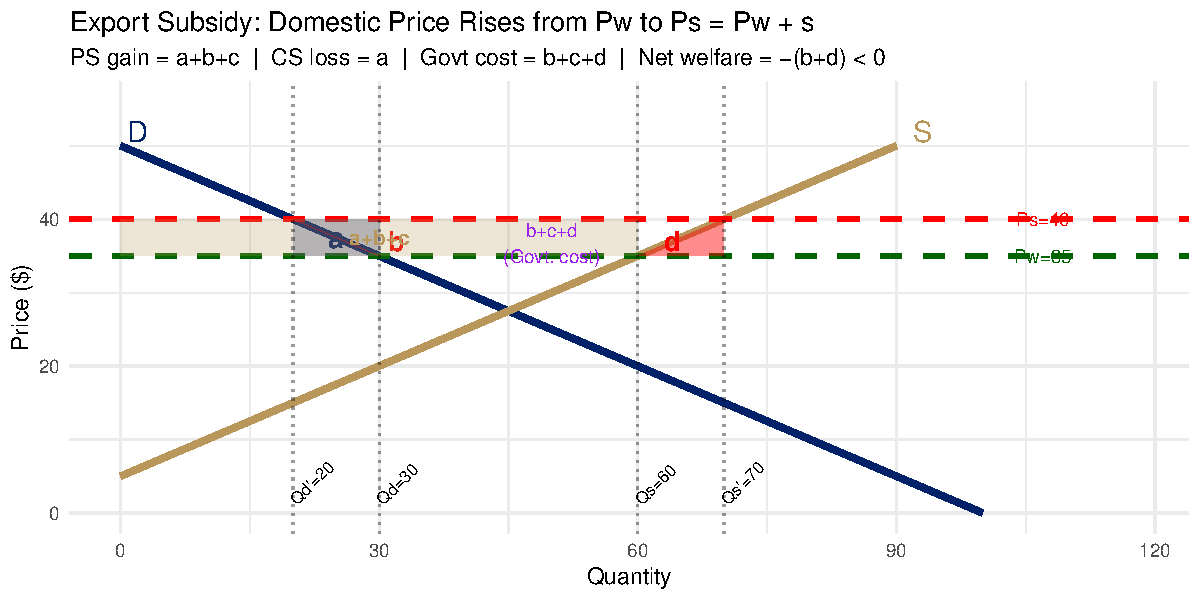
\includegraphics[keepaspectratio]{Lecture08_Protectionism_II_files/figure-beamer/fig-export-subsidy-1.pdf}}

}

\caption{Export Subsidy: Welfare Analysis for
the Exporting Country Source: Author's illustration.}
\label{fig-export-subsidy}

\end{figure}%
\end{frame}

\begin{frame}{Welfare Accounting: Export Subsidy}
\phantomsection\label{welfare-accounting-export-subsidy}
\textbf{Full decomposition (exporting country, small-country case):}

\[\Delta CS = -a \qquad \Delta PS = +(a + b + c) \qquad \text{Government cost} = -(b + c + d)\]

\[\boxed{\Delta W = -(b + d) < 0}\]

\begin{itemize}
\tightlist
\item
  \(b\) = \textbf{consumption distortion triangle}; \(d\) =
  \textbf{production distortion triangle}
\end{itemize}

\textbf{Govt cost} = \(s \times (Q_{s1} - Q_{d1})\) =
\(5 \times 50 = 250\) units

\textbf{Numerical check:}

\begin{longtable}[]{@{}lll@{}}
\toprule\noalign{}
Area & Formula & Value \\
\midrule\noalign{}
\endhead
\(a\) & \(5 \times 10\) & 50 \\
\(b\) & \(\frac{1}{2} \times 5 \times 10\) & 25 \\
\(c\) & \(5 \times (60-30)\) & 150 \\
\(d\) & \(\frac{1}{2} \times 5 \times 10\) & 25 \\
\bottomrule\noalign{}
\end{longtable}

\(\Delta W = -(b+d) = -(25+25) = -50\); Govt pays: \((b+c+d) = 200\); PS
gains: \((a+b+c) = 225\); CS loses: \(a = 50\)
\end{frame}

\begin{frame}{India's Export Subsidies: Sugar Case (WTO DS579)}
\phantomsection\label{indias-export-subsidies-sugar-case-wto-ds579}
\textbf{Background:} India's sugar support involves: SMP (Statutory
Minimum Price); FRP (Fair and Remunerative Price); production assistance
subsidy (₹13.88/quintal); MIEQ (mandated minimum export quota);
transport subsidy (₹1,000/tonne).

\textbf{WTO DS579 (2019):} Brazil, Australia, Guatemala challenged
India. \textbf{2021 Panel ruling:} India's domestic support and export
subsidies exceeded WTO AoA commitments. India appealed → pending
(Appellate Body non-functional since 2019).

\textbf{India's defence:} ``Developing countries have the right to
support food security and rural livelihoods.''

\begin{itemize}
\tightlist
\item
  AoA \textbf{de minimis} provision: Amber Box support ≤ 10\% of
  production value
\item
  Peace Clause for public stockholding; Special and Differential
  Treatment (SDT)
\end{itemize}

\textbf{Market impact:} India's subsidised sugar exports depress world
prices by an estimated 3--7\% --- harming Brazil, Thailand, and African
sugar exporters.
\end{frame}

\begin{frame}{MSP, FCI, and the Peace Clause}
\phantomsection\label{msp-fci-and-the-peace-clause}
\textbf{MSP mechanism:} CACP recommends MSP for 23 crops pre-season;
FCI/NAFED/CCI procure at MSP when market falls below; surplus procured
stock → sometimes exported.

\textbf{WTO problem:} If \(\text{MSP} > P_w\) and surplus exported at
\(P_w\):
\(\text{Implicit subsidy} = (\text{MSP} - P_w) \times Q_{\text{exported}}\)

\begin{longtable}[]{@{}llll@{}}
\toprule\noalign{}
& MSP & World price & Implicit subsidy \\
\midrule\noalign{}
\endhead
Rice & \$290 & \$450 & --- \\
Wheat & \$245 & \$260 & \textasciitilde\$15/t \\
\bottomrule\noalign{}
\end{longtable}

\textbf{Bali Peace Clause (2013):} WTO members agreed not to legally
challenge food security stockholding programmes of developing countries
--- even if support exceeds 10\% AMS limit. Condition: transparency + no
trade distortion.

\textbf{Nairobi (2015) → MC13 Abu Dhabi (2024):} Permanent solution
still pending. India insists on a permanent peace clause without the
non-distortion condition. USA/EU resist --- argue India's 800M
tonne/year FCI operations are massively trade-distorting.
\textbf{High-stakes stalemate.}
\end{frame}

\begin{frame}{What Is Dumping? Formal Definition}
\phantomsection\label{what-is-dumping-formal-definition}
\textbf{WTO Anti-Dumping Agreement (Article 2):} Dumping occurs when the
\textbf{export price} is below \textbf{normal value}:

\[\text{Normal value} = \begin{cases} P_d & \text{(home market price)} \\ P_{3C} & \text{(price to third country)} \\ COP + \text{profit} & \text{(constructed value)} \end{cases}\]

\[\text{Margin of dumping} = \text{Normal value} - P_x > 0\]

\textbf{Three conditions to impose anti-dumping duty:} (1) Dumping
margin \textgreater{} 0 (threshold: \textgreater2\%); (2) material
injury (or threat) to domestic industry; (3) causal link between dumping
and injury.

\textbf{Why would a firm dump?} Price discrimination (monopoly at home,
competitive abroad); predatory intent (eliminate competition); surplus
disposal; learning curve; input subsidy pass-through.

\textbf{Dumping ≠ comparative advantage:} Genuinely lower costs look
like dumping when compared to high-cost domestic producers.
\end{frame}

\begin{frame}{Types of Dumping}
\phantomsection\label{types-of-dumping}
\textbf{1. Sporadic Dumping:} Occasional disposal of excess inventory at
below-normal price. \emph{India example:} Bumper harvest years → surplus
wheat exported below MSP procurement price. Welfare effect on importer:
Minor, temporary.

\textbf{2. Predatory Dumping:} Strategic pricing to eliminate foreign
competition, then raise prices once rivals exit. \emph{Classic
allegation:} Chinese steel exports to India (2014--16). HRC steel
exported at \$350/tonne vs cost of \$450. Welfare effect: Temporary
gain, long-run monopolisation.

\textbf{3. Persistent Dumping:} Chronic price discrimination ---
domestic market protected → monopoly pricing at home; competitive
pricing abroad: \(P_d > P_x\) persistently.

\textbf{Arbitrage prevention:} For persistent dumping to work, the
exporter must prevent re-importation of cheaply sold exports back into
the home market. Methods: different packaging, branding, warranty
restrictions, official import controls.
\end{frame}

\begin{frame}{Dumping: Price Discrimination Diagram}
\phantomsection\label{dumping-price-discrimination-diagram}
\begin{figure}

\centering{

\pandocbounded{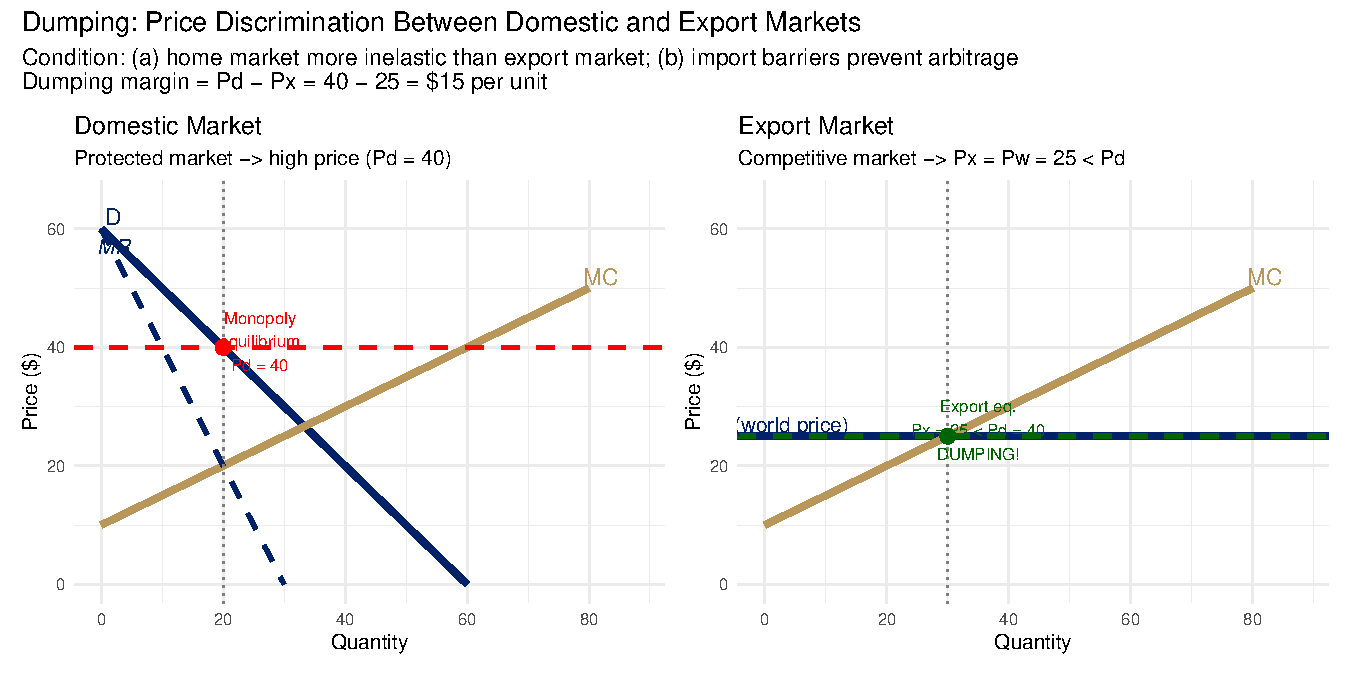
\includegraphics[keepaspectratio]{Lecture08_Protectionism_II_files/figure-beamer/fig-dumping-1.pdf}}

}

\caption{Dumping as Price Discrimination: Domestic
Monopoly Price \textgreater{} Export Price Source: Author's
illustration.}
\label{fig-dumping}

\end{figure}%
\end{frame}

\begin{frame}{Dumping: Formal Condition and Anti-Dumping Duty}
\phantomsection\label{dumping-formal-condition-and-anti-dumping-duty}
\textbf{Dumping condition (price discrimination version):}

\[P_x < P_d \quad \Leftrightarrow \quad \frac{P_x}{P_d} < 1\]

In profit-maximising terms:
\(P_d \left(1 - \frac{1}{|e_d|}\right) = P_x \left(1 - \frac{1}{|e_x|}\right)\)

If \(|e_x| > |e_d|\) (export market more elastic), then \(P_x < P_d\). ✓

\textbf{Anti-dumping duty (ADD):}
\(\text{ADD} = P_d - P_x = \text{margin of dumping}\) --- raises \(P_x\)
back toward \(P_d\).

\textbf{Welfare effects of ADD for importing country:}

\begin{longtable}[]{@{}ll@{}}
\toprule\noalign{}
Effect & Direction \\
\midrule\noalign{}
\endhead
Consumer surplus & Falls (price rises) \\
Producer surplus & Rises (domestic producers protected) \\
Govt revenue (ADD) & Rises \\
Net welfare & Ambiguous --- DWL likely \\
\bottomrule\noalign{}
\end{longtable}

\(\Delta W = -b - d + \text{PS gain}\) --- if domestic production is
efficient, \(\Delta W\) may be positive; if ADD is protectionist,
\(\Delta W < 0\).
\end{frame}

\begin{frame}{India's Anti-Dumping Experience}
\phantomsection\label{indias-anti-dumping-experience}
\begin{figure}

\centering{

\pandocbounded{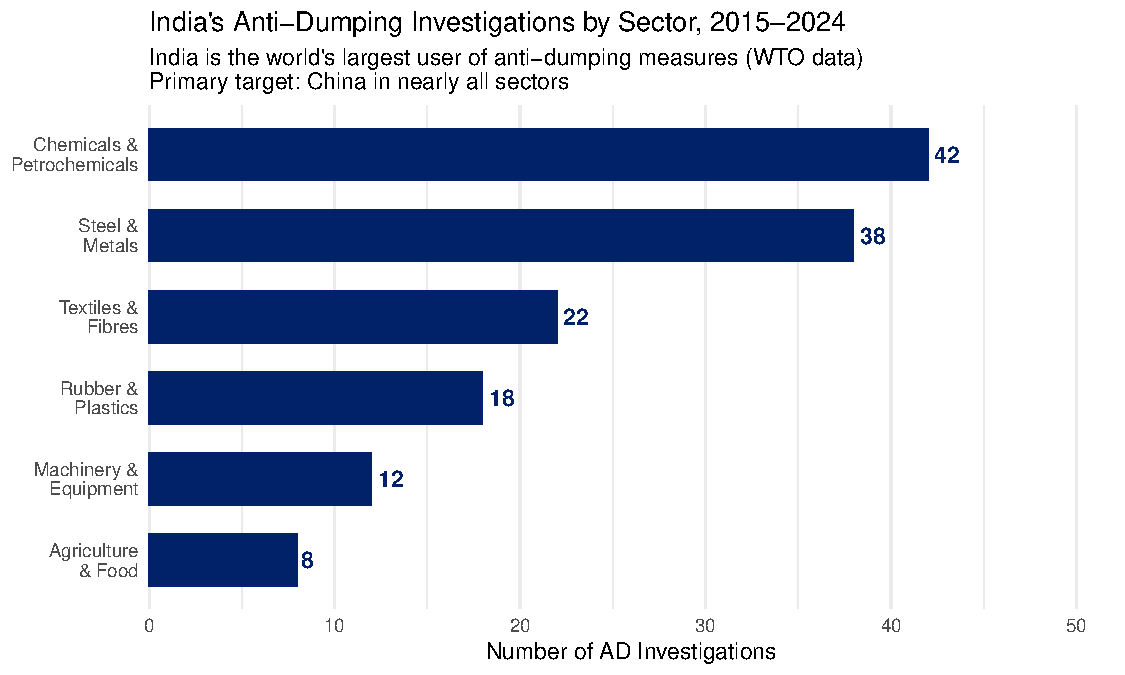
\includegraphics[keepaspectratio]{Lecture08_Protectionism_II_files/figure-beamer/fig-india-add-1.pdf}}

}

\caption{India: Anti-Dumping Investigations
Initiated by Sector (2015--2024) Source: DGTR, Ministry of Commerce,
GoI.}
\label{fig-india-add}

\end{figure}%
\end{frame}

\begin{frame}{Indian Agriculture Facing Dumping Allegations Abroad}
\phantomsection\label{indian-agriculture-facing-dumping-allegations-abroad}
\textbf{Indian shrimp exports (USA):} USA imposed CVD + AD duties on
Indian shrimp (2003, 2013, 2023); margin of dumping: 4.98--6.3\% (2023
review). India's argument: low costs reflect \textbf{genuine comparative
advantage} (labour, aquaculture efficiency), not subsidies.

\textbf{Indian basmati rice:} EU phytosanitary restrictions (pesticide
MRLs) periodically block Indian exports --- not formal AD, but
equivalent effect.

\textbf{Indian buffalo meat:} EU AD allegations (cold cuts); AD margin
investigations initiated 2021. India's position: lowest-cost producer
due to cattle by-product economics.

\textbf{Comparative advantage vs.~dumping:} A developing country with
genuinely low costs will \emph{appear} to dump when compared to
high-cost producers in developed countries.
\(P_{\text{India}} < P_{\text{USA}} \not\Rightarrow \text{dumping}\).
Dumping requires \(P_{\text{export}} < \text{normal value}\). In
practice, AD is often used as disguised protectionism.
\end{frame}

\begin{frame}{VERs --- Quotas Imposed ``Voluntarily'' by Exporters}
\phantomsection\label{vers-quotas-imposed-voluntarily-by-exporters}
A \textbf{Voluntary Export Restraint (VER)} is an agreement where the
\emph{exporting} country ``voluntarily'' limits its exports --- usually
under diplomatic pressure.

\textbf{Why ``voluntary''?} Importing country threatens worse action;
exporter prefers VER --- quota rent goes to \emph{foreign exporter};
both governments prefer quiet bilateral deal to WTO dispute.

\textbf{Classic example:} Japan--USA auto VER (1981): Japan agreed to
limit car exports at 1.68M units/year. Toyota, Honda captured quota rent
→ funded quality upgrading → ultimately made Japanese cars stronger.

\textbf{VER vs.~Tariff vs.~Quota:}

\begin{longtable}[]{@{}lll@{}}
\toprule\noalign{}
Instrument & Who gets rent? & WTO-legal? \\
\midrule\noalign{}
\endhead
Tariff & Importing govt & Yes \\
Quota & Licence holders & Yes (with rules) \\
VER & \textbf{Foreign exporter} & \textbf{No (UR banned)} \\
\bottomrule\noalign{}
\end{longtable}

Uruguay Round (1994): VERs explicitly prohibited under WTO safeguards
agreement. But ``Orderly Marketing Arrangements'' and ``grey area''
bilateral deals persist under different names.
\end{frame}

\begin{frame}{VER Welfare Analysis}
\phantomsection\label{ver-welfare-analysis}
A VER is economically equivalent to an import quota --- but worse for
the importing country:

\textbf{Standard quota welfare:}
\(\Delta W_{\text{import country}} = -(b + d) + c\) where \(c\) = quota
rent captured by licence holders.

\textbf{VER welfare:}
\(\Delta W_{\text{import country}} = -(b + c + d)\) because \(c\) =
quota rent goes to \textbf{foreign exporters}, not domestic licence
holders.

\[\boxed{\text{VER strictly worse than equivalent quota for importing country}}\]

\textbf{Numerical example:} Suppose VER restricts imports to
\(\bar{M}\).

\begin{itemize}
\tightlist
\item
  \(b\) = production distortion:
  \(\frac{1}{2}(P_d - P_w) \cdot \Delta Q_s\)
\item
  \(c\) = quota rent: \((P_d - P_w) \cdot \bar{M}\)
\item
  \(d\) = consumption distortion:
  \(\frac{1}{2}(P_d - P_w) \cdot \Delta Q_d\)
\end{itemize}

Under tariff: \(\Delta W_{\text{tariff}} = -(b+d) + t \cdot M\); Under
VER: \(\Delta W_{\text{VER}} = -(b+c+d) < \Delta W_{\text{tariff}}\)
\end{frame}

\begin{frame}{What Is a Cartel? Conditions for Success}
\phantomsection\label{what-is-a-cartel-conditions-for-success}
A \textbf{cartel} is a formal/informal agreement among producers to
restrict output, fix prices, or divide markets.
\textbf{Profit-maximising cartel acts as a monopolist:}
\(MR = MC \Rightarrow Q^* < Q_{\text{competitive}}, P^* > P_{\text{competitive}}\);
world welfare loss = \(-(b + d)\).

\textbf{Conditions for cartel success:} (1) Concentrated supply; (2)
inelastic demand; (3) discipline (no cheating); (4) barriers to entry;
(5) product homogeneity.

\textbf{OPEC as reference:} OPEC controls \textasciitilde38\% of world
oil supply. Production cuts (2022--23) raised Brent crude from \$75 to
\$120/barrel.

\textbf{Agricultural cartels rarely succeed:} Many producers; many
substitutes (rice ↔ wheat ↔ maize); perishable goods; low entry
barriers; political pressure to sell for domestic food security.

\[\Rightarrow \text{Agricultural cartels are theoretically possible, practically unstable}\]
\end{frame}

\begin{frame}{International Commodity Agreements (ICAs): instruments}
\phantomsection\label{international-commodity-agreements-icas-instruments}
ICAs are multilateral attempts to \textbf{stabilise commodity prices}.

\begin{itemize}
\tightlist
\item
  \textbf{Buffer stocks:} buy when price is ``too low'', sell when ``too
  high''
\item
  \textbf{Export quotas:} allocate export shares across members
\item
  \textbf{Long-term contracts:} guarantee volumes at agreed prices
\item
  \textbf{Works best when:} large market share, homogeneous commodity,
  credible financing
\item
  \textbf{Key caution:} agriculture has close substitutes → stability is
  hard
\end{itemize}
\end{frame}

\begin{frame}{Why ICAs fail in practice}
\phantomsection\label{why-icas-fail-in-practice}
\begin{itemize}
\tightlist
\item
  \textbf{Free-rider problem:} non-members expand exports when prices
  rise
\item
  \textbf{Cheating:} members secretly exceed quotas
\item
  \textbf{Financing constraint:} buffer stocks become fiscally
  unsustainable
\item
  \textbf{Substitutes + tech change:} demand shifts undermine price
  bands
\item
  \textbf{North--South conflict:} producers want high prices; consumers
  want low prices
\end{itemize}

\note{UNCTAD's Integrated Programme for Commodities (1976) proposed 18
ICAs; most collapsed within \textasciitilde15 years.}
\end{frame}

\begin{frame}{History of International Commodity Agreements}
\phantomsection\label{history-of-international-commodity-agreements}
\textbf{Examples and outcomes:}

\begin{itemize}
\tightlist
\item
  Coffee (ICO): collapsed (free-riding)
\item
  Tin (ITA): collapsed (buffer-stock bankruptcy)
\item
  Sugar (ISA): weakened (price provisions abandoned)
\item
  Jute (IJO): wound down (2014)
\item
  Cocoa (ICCO): repeated failures; restructured
\end{itemize}
\end{frame}

\begin{frame}{Tin crisis (1985): why buffer stocks fail}
\phantomsection\label{tin-crisis-1985-why-buffer-stocks-fail}
\begin{itemize}
\tightlist
\item
  Prices fell sharply; buffer-stock manager ran out of funds
\item
  Agreement collapsed and disrupted the tin market
\item
  Prices plunged by about \textbf{40\%} in days
\item
  Price bands require \textbf{credible financing} (hard politically)
\item
  Takeaway: ICAs are fragile when compliance and funding are weak
\end{itemize}
\end{frame}

\begin{frame}{India's Rice Export Ban (2023): Unilateral Market Power}
\phantomsection\label{indias-rice-export-ban-2023-unilateral-market-power}
\begin{columns}[T]
\begin{column}{0.55\linewidth}
\textbf{India's rice export market position:}

\begin{itemize}
\tightlist
\item
  World's largest rice exporter: \textbf{\textasciitilde40\% of global
  rice trade} (FY2022-23: 22 MMT)
\item
  Dominant in non-basmati white rice: \textasciitilde60\% of world
  market
\end{itemize}

\textbf{August 2023 policy actions:}

\begin{enumerate}
\tightlist
\item
  \textbf{Ban} on non-basmati white rice exports
\item
  \textbf{20\% export duty} on parboiled rice
\item
  \textbf{\$1,200/tonne MEP} on basmati rice
\end{enumerate}

\textbf{Immediate market impact:}

\begin{itemize}
\tightlist
\item
  World rice prices surged \textbf{20--30\%} in 2 months
\item
  Philippines, Indonesia, West Africa most affected
\item
  Bangladesh, Senegal faced acute food security risks
\end{itemize}
\end{column}

\begin{column}{0.45\linewidth}
\textbf{Economic analysis:}

With 40\% world market share, India has significant
\textbf{monopsonist/monopolist power} in rice --- analogous to a cartel
without formal coordination.

\textbf{India's justification:} WTO Article XI permits export
restrictions for food security.

\textbf{Counter-argument:} When a single country controls 40\% of world
supply, its ``domestic food security'' restriction \emph{is} a global
food security threat.

\[P_{\text{world}} \uparrow 25\% \Rightarrow \text{500M+ people in importing countries pay more for food}\]

\textbf{Lesson:} Market concentration creates policy power --- with
global externalities.
\end{column}
\end{columns}
\end{frame}

\begin{frame}{Strategic Trade Policy and Infant Industry Argument}
\phantomsection\label{strategic-trade-policy-and-infant-industry-argument}
\begin{columns}[T]
\begin{column}{0.55\linewidth}
\textbf{Infant industry argument} (Hamilton 1791; List 1841):

Temporary protection allows a new industry to: 1. Achieve economies of
scale 2. Move down the learning curve 3. Become internationally
competitive

\textbf{Learning-by-doing model:}

\[C_t = C_0 \cdot e^{-\lambda Q_t^{\text{cumulative}}}\]

where \(\lambda\) = learning rate. Production cost falls with cumulative
experience.

\textbf{Protection justified if:}

\[\sum_{t=0}^{T} \frac{\text{PS gain}_t - \text{CS loss}_t}{(1+r)^t} > 0\]

i.e., present value of future gains exceeds current protection costs.
\end{column}

\begin{column}{0.45\linewidth}
\textbf{India examples:}

\textbf{Edible oil (1970s-90s):} Heavy protection of domestic oilseed
processing. - Result: Yellow revolution (oilseed production rose) - But
productivity gains lagged; protection lasted too long

\textbf{Sugar industry:} - 100+ years of protection - Still high-cost
producer by global standards - Protection → no incentive to compete

\textbf{Counter-argument to infant industry:} If the learning curve is
genuinely valuable, private capital should finance it. Government
intervention needed only if: (a) capital market failure, or (b) positive
spillovers (externalities) that private firm cannot capture.

\[\text{Subsidy justified} \iff \text{market failure exists}\]
\end{column}
\end{columns}
\end{frame}

\begin{frame}{WTO Disciplines: Key Rules Summary}
\phantomsection\label{wto-disciplines-key-rules-summary}
\begin{columns}[T]
\begin{column}{0.55\linewidth}
\begin{longtable}[]{@{}
  >{\raggedright\arraybackslash}p{(\linewidth - 2\tabcolsep) * \real{0.5000}}
  >{\raggedright\arraybackslash}p{(\linewidth - 2\tabcolsep) * \real{0.5000}}@{}}
\toprule\noalign{}
\begin{minipage}[b]{\linewidth}\raggedright
Instrument
\end{minipage} & \begin{minipage}[b]{\linewidth}\raggedright
WTO status
\end{minipage} \\
\midrule\noalign{}
\endhead
Export subsidies (developed) & \textbf{Prohibited} (MC10 Nairobi
2015) \\
Export subsidies (developing) & Phased out \\
Domestic subsidies (Amber Box) & Limited by AMS cap \\
Anti-dumping duties & Permitted (ADA) \\
Countervailing duties & Permitted (SCMA) \\
VERs & \textbf{Prohibited} (Art. 11, SA) \\
Export restrictions (quotas/bans) & Permitted for food security (Art.
XI:2) \\
Export cartels & No explicit WTO rule --- governed by domestic
competition law \\
\bottomrule\noalign{}
\end{longtable}

\note{\textbf{Key gaps in WTO rules:} - Export restrictions
(increasingly used by India, China, Indonesia) - State trading
enterprises (FCI, COFCO) - Input subsidies to developing countries}
\end{column}

\begin{column}{0.45\linewidth}
\textbf{Countervailing Duties (CVD):}

CVDs target foreign \emph{subsidies} (not dumping):

\[\text{CVD} = \text{amount of foreign subsidy}\]

Condition: subsidy is ``specific'' (to a firm/industry) AND causes
material injury.

\textbf{SCMA Agreement} governs CVDs.

India has faced CVDs primarily from USA on shrimp, steel, and
pharmaceutical exports.

India has used CVDs less frequently than AD duties --- but use is
growing as India targets subsidised Chinese and EU agricultural exports.
\end{column}
\end{columns}
\end{frame}

\begin{frame}{Key Takeaways: Lecture 8}
\phantomsection\label{key-takeaways-lecture-8}
\textbf{1. Export subsidies} distort production and trade; harm
importing-country farmers; impose fiscal costs on the subsidising
government. Net welfare effect for exporting country:
\(\Delta W = -(b+d) < 0\).

\textbf{2. India's MSP + FCI procurement} creates implicit export
subsidies when procurement prices exceed world prices. Sugar WTO dispute
(DS579) shows WTO's limits in disciplining developing country support.

\textbf{3. Dumping} = selling below normal value. Formal condition:
\(P_x < P_d\) or \(P_x < AVC\). India is the world's largest AD user;
but Indian exporters also face spurious AD allegations that confuse
genuine comparative advantage with dumping.

\textbf{4. VERs} are strictly worse than equivalent tariffs for the
importing country --- quota rent is transferred abroad:
\(\Delta W_{\text{VER}} = -(b+c+d) < -(b+d) = \Delta W_{\text{tariff}}\).

\textbf{5. Agricultural cartels} fail because: many producers, many
substitutes, perishable goods, easy entry. But India's unilateral market
power in rice (40\% of world exports) achieves cartel-like effects
without formal coordination.

\note{\textbf{6. WTO disciplines} have significant gaps --- particularly
on export restrictions, state trading, and developing-country input
subsidies. This creates ongoing North-South tensions.}
\end{frame}

\begin{frame}{Next Lecture Preview}
\phantomsection\label{next-lecture-preview}
\textbf{Lecture 9 --- Balance of Trade \& Balance of Payments}
\emph{June 20, 2026}

\begin{itemize}
\tightlist
\item
  What is the BoP? Three-account structure and accounting identity
\item
  National income identity approach:
  \(\text{CA} = Y - A = S - I + (T - G)\)
\item
  India's current account: merchandise deficit, services surplus,
  remittances
\item
  Capital and financial account: FDI vs FPI, RBI reserve management
\item
  Marshall-Lerner condition: \(|e_X| + |e_M| > 1\)
\end{itemize}

\note{\begin{itemize}
\tightlist
\item
  J-curve effect: why depreciation worsens trade balance before
  improving it
\item
  India's 1991 BoP crisis: \$1.2B reserves, gold pledging, IMF
  conditionality
\item
  India FY2024 external sector assessment
\end{itemize}

\textbf{Preparation:} Read Salvatore Ch. 12--13; RBI Annual Report
2023-24, External Sector chapter. Review IS-LM model --- we will use it
to analyse policy responses to BoP disequilibrium.}
\end{frame}

\section{Appendix}\label{appendix}

\begin{frame}{Additional Resources}
\phantomsection\label{additional-resources}
\begin{columns}[T]
\begin{column}{0.5\linewidth}
\textbf{Further Reading}

\begin{itemize}
\tightlist
\item
  \emph{International Economics} --- Salvatore (Ch. 9-11)
\item
  \emph{International Economics} --- Appleyard \& Field (Ch. 9-11)
\item
  RBI/DGCI\&S/APEDA databases for latest data
\end{itemize}
\end{column}

\begin{column}{0.5\linewidth}
\textbf{Key Data Sources}

\begin{itemize}
\tightlist
\item
  DGCI\&S: India's merchandise trade
\item
  RBI: Balance of payments data\\
\item
  APEDA: Agricultural export statistics
\item
  WTO: Tariff and trade databases
\end{itemize}
\end{column}
\end{columns}
\end{frame}




\end{document}
